\documentclass[10pt,a4paper]{article}
\usepackage[margin=2.0cm]{geometry}
\usepackage[T1]{fontenc}
\usepackage{lmodern}
\usepackage{microtype}
\usepackage[table]{xcolor}
\usepackage{booktabs,array}
\usepackage{tabularx}
\usepackage{amsmath,amssymb}
\usepackage{graphicx}
\usepackage{tikz}
\usetikzlibrary{arrows.meta,positioning,calc}
\usepackage{float}
\usepackage{placeins}
\usepackage{xr-hyper}
\usepackage[hidelinks]{hyperref}
\externaldocument[main-]{contextual_sparse_etm_report}[contextual_sparse_etm_report.pdf]
\usepackage{enumitem}
\usepackage{fancyhdr}
\definecolor{accent}{HTML}{1D4ED8}
\definecolor{accentlight}{HTML}{DBEAFE}
\definecolor{softgray}{HTML}{F3F4F6}
\definecolor{lossgold}{HTML}{C6922F}
\hypersetup{colorlinks=true,linkcolor=accent,urlcolor=accent,citecolor=accent,
pdftitle={Supplementary Information: Neural Topic Models for Mass Spectra}}
% Current-model numbers come only from the selected whole-spectrum model.
% Generated: chosen full-document model; validation only.
\newcommand{\CurrentEvaluableMean}{665.7}
\newcommand{\CurrentEvaluableSD}{7.6}
\newcommand{\CurrentUsefulMean}{390.7}
\newcommand{\CurrentUsefulSD}{2.1}
\newcommand{\CurrentSOSMean}{0.629}
\newcommand{\CurrentSOSSD}{0.002}
\newcommand{\CurrentNLLMean}{9.525}
\newcommand{\CurrentNLLSD}{0.023}
\newcommand{\CurrentEffectiveMean}{3.72}
\newcommand{\CurrentEffectiveSD}{0.03}
\newcommand{\CurrentWinnersMean}{807.3}
\newcommand{\CurrentWinnersSD}{9.1}
\newcommand{\ReferenceLDAEvaluable}{578.0}
\newcommand{\ReferenceLDAEvaluableSD}{5.0}
\newcommand{\ReferenceLDAUseful}{351.7}
\newcommand{\ReferenceLDAUsefulSD}{7.0}
\newcommand{\ReferenceLDASOS}{0.639}
\newcommand{\ReferenceLDASOSSD}{0.003}
\newcommand{\ReferenceLDANLL}{9.693}
\newcommand{\ReferenceLDANLLSD}{0.004}
\newcommand{\ReferenceLDAEffective}{9.26}
\newcommand{\ReferenceLDAEffectiveSD}{0.09}
\newcommand{\ReferenceCanonicalEvaluable}{202.7}
\newcommand{\ReferenceCanonicalEvaluableSD}{5.5}
\newcommand{\ReferenceCanonicalUseful}{125.0}
\newcommand{\ReferenceCanonicalUsefulSD}{6.1}
\newcommand{\ReferenceCanonicalSOS}{0.637}
\newcommand{\ReferenceCanonicalSOSSD}{0.006}
\newcommand{\ReferenceCanonicalNLL}{8.707}
\newcommand{\ReferenceCanonicalNLLSD}{0.029}
\newcommand{\ReferenceCanonicalEffective}{40.75}
\newcommand{\ReferenceCanonicalEffectiveSD}{1.09}
\newcommand{\CurrentUsefulDifference}{+39.0}

\newcommand{\ChemPrimaryStrata}{158}
\newcommand{\ChemFixedCompounds}{64}
\newcommand{\ChemSelectedEligibleMin}{657}
\newcommand{\ChemSelectedEligibleMax}{671}
\newcommand{\ChemSelectedSupportedMin}{799}
\newcommand{\ChemSelectedSupportedMax}{817}
\newcommand{\ChemLDAEligibleMin}{573}
\newcommand{\ChemLDAEligibleMax}{583}
\newcommand{\ChemLDASupportedMin}{933}
\newcommand{\ChemLDASupportedMax}{959}
\newcommand{\ChemLDASingletonEligible}{75.3}
\newcommand{\ChemLDARecurring}{502.7}
\newcommand{\ChemLDARecurringSD}{13.0}
\newcommand{\ChemLDASingleton}{132.7}
\newcommand{\ChemLDASingletonSD}{12.9}
\newcommand{\ChemLDABackground}{0.604}
\newcommand{\ChemLDABackgroundSD}{0.002}
\newcommand{\ChemLDAExcess}{0.035}
\newcommand{\ChemLDAExcessSD}{0.001}
\newcommand{\ChemLDASOSTopics}{9.7}
\newcommand{\ChemLDASOSTopicsSD}{3.5}
\newcommand{\ChemLDAFeatureTopics}{12.0}
\newcommand{\ChemLDAFeatureTopicsSD}{3.0}
\newcommand{\ChemSelectedSingletonEligible}{151.0}
\newcommand{\ChemSelectedRecurring}{514.7}
\newcommand{\ChemSelectedRecurringSD}{14.2}
\newcommand{\ChemSelectedSingleton}{197.0}
\newcommand{\ChemSelectedSingletonSD}{8.9}
\newcommand{\ChemSelectedBackground}{0.594}
\newcommand{\ChemSelectedBackgroundSD}{0.003}
\newcommand{\ChemSelectedExcess}{0.035}
\newcommand{\ChemSelectedExcessSD}{0.003}
\newcommand{\ChemSelectedSOSTopics}{10.7}
\newcommand{\ChemSelectedSOSTopicsSD}{1.5}
\newcommand{\ChemSelectedFeatureTopics}{10.0}
\newcommand{\ChemSelectedFeatureTopicsSD}{1.7}
\newcommand{\ChemLDAScaffoldExcess}{0.029}
\newcommand{\ChemLDAScaffoldFeatureTopics}{3.0}
\newcommand{\ChemSelectedScaffoldExcess}{0.032}
\newcommand{\ChemSelectedScaffoldFeatureTopics}{3.0}
\newcommand{\ChemSelectedMatchMedian}{0.625}
\newcommand{\ChemSelectedReciprocal}{0.673}
\newcommand{\ChemSelectedCompoundMatch}{0.012}
\newcommand{\ChemSelectedRedundantMedian}{0.093}
\newcommand{\ChemSelectedRepeatedMAG}{96.3}
\newcommand{\ChemSelectedRepeatedMAGPercent}{11.9}
\newcommand{\ChemSelectedReferenceMedian}{0.201}
\newcommand{\ChemSelectedReferenceOverlap}{0.066}
\newcommand{\ChemSelectedReferenceAnyOverlap}{662.0}
\newcommand{\ChemLDAMatchMedian}{0.529}
\newcommand{\ChemLDAReciprocal}{0.666}
\newcommand{\ChemLDACompoundMatch}{0.000}
\newcommand{\ChemLDARedundantMedian}{0.025}
\newcommand{\ChemLDARepeatedMAG}{47.7}
\newcommand{\ChemLDARepeatedMAGPercent}{7.8}
\newcommand{\ChemLDAReferenceMedian}{0.188}
\newcommand{\ChemLDAReferenceOverlap}{0.069}
\newcommand{\ChemLDAReferenceAnyOverlap}{531.3}
\newcommand{\ChemCrossMatchMedian}{0.404}
\newcommand{\ChemRawReferences}{255}
\newcommand{\ChemUniqueReferences}{234}
\newcommand{\ChemScorableReferences}{234}
\newcommand{\ChemExcludedReferences}{0}
\newcommand{\ChemConflictingReferences}{8}

\newcommand{\OverlapNNChemicalDefined}{3,088}
\newcommand{\OverlapNNChemicalUndefined}{0}
\newcommand{\OverlapNNAllCos}{0.650}
\newcommand{\OverlapNNRecurringCos}{0.625}
\newcommand{\OverlapNNCompound}{0.171}
\newcommand{\OverlapNNChemical}{0.423}
\newcommand{\OverlapNNFragment}{0.718}
\newcommand{\OverlapNNLoss}{0.379}
\newcommand{\OverlapNNChannelCos}{0.508}
\newcommand{\OverlapNNNoMAGFilterCos}{0.635}
\newcommand{\OverlapNLChemicalDefined}{4,631}
\newcommand{\OverlapNLChemicalUndefined}{1}
\newcommand{\OverlapNLAllCos}{0.454}
\newcommand{\OverlapNLRecurringCos}{0.420}
\newcommand{\OverlapNLCompound}{0.075}
\newcommand{\OverlapNLChemical}{0.260}
\newcommand{\OverlapNLFragment}{0.550}
\newcommand{\OverlapNLLoss}{0.006}
\newcommand{\OverlapNLChannelCos}{0.339}
\newcommand{\OverlapNLNoMAGFilterCos}{0.516}
\newcommand{\OverlapLNChemicalDefined}{4,521}
\newcommand{\OverlapLNChemicalUndefined}{3}
\newcommand{\OverlapLNAllCos}{0.454}
\newcommand{\OverlapLNRecurringCos}{0.460}
\newcommand{\OverlapLNCompound}{0.089}
\newcommand{\OverlapLNChemical}{0.307}
\newcommand{\OverlapLNFragment}{0.547}
\newcommand{\OverlapLNLoss}{0.007}
\newcommand{\OverlapLNChannelCos}{0.337}
\newcommand{\OverlapLNNoMAGFilterCos}{0.403}
\newcommand{\OverlapLLChemicalDefined}{3,011}
\newcommand{\OverlapLLChemicalUndefined}{5}
\newcommand{\OverlapLLAllCos}{0.547}
\newcommand{\OverlapLLRecurringCos}{0.525}
\newcommand{\OverlapLLCompound}{0.167}
\newcommand{\OverlapLLChemical}{0.382}
\newcommand{\OverlapLLFragment}{0.705}
\newcommand{\OverlapLLLoss}{0.003}
\newcommand{\OverlapLLChannelCos}{0.394}
\newcommand{\OverlapLLNoMAGFilterCos}{0.524}
\newcommand{\OverlapMedianCos}{0.422}
\newcommand{\OverlapMedianSecondCos}{0.107}
\newcommand{\OverlapMedianFragmentShared}{1}
\newcommand{\OverlapMedianLossShared}{0}
\newcommand{\OverlapUpperCos}{0.887}
\newcommand{\OverlapUpperSecondCos}{0.087}
\newcommand{\OverlapUpperFragmentShared}{2}
\newcommand{\OverlapUpperLossShared}{0}
\newcommand{\OverlapMultipleCos}{0.522}
\newcommand{\OverlapMultipleSecondCos}{0.324}
\newcommand{\OverlapMultipleFragmentShared}{5}
\newcommand{\OverlapMultipleLossShared}{0}
\newcommand{\OverlapMultipleSecondFragmentShared}{3}
\newcommand{\OverlapMultipleSecondLossShared}{0}

\pagestyle{fancy}
\fancyhf{}
\setlength{\headheight}{14pt}
\setlength{\headsep}{18pt}
\cfoot{\thepage}
\renewcommand{\headrulewidth}{0pt}
\fancypagestyle{plain}{\fancyhf{}\cfoot{\thepage}\renewcommand{\headrulewidth}{0pt}}
\setlist{nosep,leftmargin=*}
\newcommand{\softmax}{\operatorname{softmax}}
\newcommand{\normalize}{\operatorname{normalize}}
\newcommand{\entmax}{\operatorname{entmax}_{1.5}}
\newcommand{\KL}{\operatorname{KL}}
\newcommand{\ctxscale}{\lambda_{\mathrm{ctx}}}
\tikzset{
  modelnode/.style={draw=black!55,rounded corners=2pt,align=center,
    minimum height=1.05cm,inner sep=3pt,font=\footnotesize,text width=2.35cm},
  dataflow/.style={-{Latex[length=2mm]},line width=0.55pt,draw=black!70},
  pipelinebox/.style={draw=black!55,fill=softgray,rounded corners=2pt,
    align=center,minimum height=1.2cm,text width=2.5cm,inner sep=3pt,font=\scriptsize}
}

\renewcommand{\thesection}{S\arabic{section}}
\renewcommand{\theequation}{S\arabic{equation}}
\renewcommand{\thefigure}{S\arabic{figure}}
\renewcommand{\thetable}{S\arabic{table}}
\renewcommand{\thepage}{S\arabic{page}}
\title{Supplementary Information\\[4pt]\large Discovering Molecular Substructures from Mass Spectra\\with Neural Topic Models}
\author{}
\date{}
\begin{document}
\maketitle
This document accompanies the
\href{contextual_sparse_etm_report.pdf}{main paper}. It preserves the full
model equations, evaluation protocols and reproducibility record underlying
the shorter explanations there. S-prefixed section, equation, figure and table
numbers refer to this supplement. References to main figures open the companion
PDF; keep both files in the same directory.
\setcounter{tocdepth}{1}
\tableofcontents
\clearpage
\section{Notation and spectral data}
\label{sec:data}
\subsection{Notation and scope}

Table~\ref{tab:notation} defines the main indices and quantities before the
model equations. A word index identifies a \emph{vocabulary type}; a token is
one count-weighted copy of that word, not necessarily a distinct physical
peak. Throughout, sums over $w$ or $v$ cover the vocabulary unless a channel
or evaluation subset is specified, and sums over $k$ or $j$ cover all topics.
Subscript $d$ denotes a spectrum, never a dataset or training repetition.

\begin{table}[H]
\centering\small
\caption{Core notation. Auxiliary quantities are defined where introduced.}
\label{tab:notation}
\renewcommand{\arraystretch}{1.12}
\begin{tabularx}{\textwidth}{@{}p{3.6cm}X@{}}
\toprule
Symbol & Meaning and dimensions \\
\midrule
$D$; $d=1,\ldots,D$ & Number of spectra in the stated partition; spectrum index. \\
$V$; $w,v=1,\ldots,V$ & Vocabulary size; spectral-word indices. \\
$K$; $k,j=1,\ldots,K$ & Number of fitted topics; topic indices. \\
$E$; $\mathcal V_F,\mathcal V_L$ & Embedding dimension; disjoint fragment and loss vocabularies whose union is the full vocabulary. \\
$c_d,x_d\in\mathbb R^V$; $N_d$ & Word pseudo-count vector, normalized encoder input, and total in-vocabulary count. \\
$\rho_w,\alpha_k\in\mathbb R^E$ & Fixed word vector and learned topic vector; tables have shapes $V\times E$ and $K\times E$. \\
$\beta\in\mathbb R^{K\times V}$; $\theta_d\in\mathbb R^K$ & Topic--word probabilities and spectrum-level topic proportions; each row/vector sums to one. \\
$z_d,m_d,\ell_d\in\mathbb R^K$ & Gaussian latent vector, corrected posterior mean, and log variance. \\
$\phi$; $I_K$ & MLP parameters; $K\times K$ identity matrix (not peak intensity). \\
$s_d,h_{dw}\in\mathbb R^E$ & Whole-spectrum mean embedding and contextualized word direction. \\
$\ctxscale\in\mathbb R$ & One learned context-strength scalar, distinct from count $c_{dw}$. \\
$r_d,o_d\in\mathbb R^K$ & Pooled topic evidence and its centered-log mean correction. \\
\bottomrule
\end{tabularx}
\end{table}

Vector exponentials and logarithms operate elementwise; $\operatorname{diag}$
forms a diagonal matrix, and $\odot$ denotes elementwise multiplication.
The notation $\mathcal N$ denotes a Gaussian distribution. A probability
vector lies on the simplex: its entries are nonnegative and sum to one.
Hats on embedding vectors mean unit normalization; hats on inferred mixtures
mean deterministic estimates, as defined below.

\subsection{Spectral representation and data preparation}

\paragraph{Real reference spectra.}
MS$^{n}$Lib is an open library of reference-standard fragmentation spectra,
including multi-stage measurements \cite{brungs2025}. We use the
positive-ion-mode benchmark subset distributed in Mascot Generic Format
(MGF) with the MS2LDA 2.0 data and models \cite{msnlibdata}, not the entire
MS$^{n}$Lib collection. An MGF record supplies a precursor $m/z$, a list of
fragment $m/z$ values and intensities, and metadata linking the spectrum to
its known molecule. Known structures permit chemically grouped splitting
and evaluation; they are not ground-truth labels for every latent motif.

\paragraph{Peak filtering and intensity representation.}
The input contains 41,568 spectra. Intensities are divided by the largest
intensity within each spectrum; peaks outside $m/z\in(0,2000]$ or normalized
intensity $[0.01,1]$ are removed. At most the 1,000 most intense peaks are
retained, and spectra with fewer than five retained peaks are discarded.
This leaves 38,888 spectra. Normalizing each spectrum to its strongest peak
makes the representation
independent of overall signal scale; the intensity cutoff suppresses weak
peaks, the peak cap bounds document size, and the minimum-peak rule excludes
spectra with too few peaks for the analysis. Weaker peaks may still carry
structural information; these filtering choices define the benchmark input.

\paragraph{From peaks to spectral words.}
Each retained physical peak generates a fragment word and, if precursor-minus-peak
$m/z$ exceeds 0.01, a neutral-loss word. Here ``loss'' follows the benchmark's
precursor-minus-fragment convention; it does not infer charge-resolved
neutral compositions. Mass values are rounded to two decimal
places, for example \texttt{frag@70.04} and \texttt{loss@162.05}.
Normalized peak intensity $I$ contributes $\operatorname{round}(100I)$ copies
of each applicable word. Let $c_{dw}$ be the resulting pseudo-count of word
$w$ in spectrum $d$ and $N_d=\sum_w c_{dw}$. The normalized input is
\[
 x_{dw}=\begin{cases}c_{dw}/N_d,&N_d>0,\\0,&N_d=0.\end{cases}
\]
The encoder receives $x_d$; the reconstruction term uses raw counts $c_d$.
Counts are summed when multiple peaks yield the same word. They encode
discretized relative intensity, not independent ion counts or a calibrated
noise model. For example, a peak at $m/z=60.00$ from a precursor at
$m/z=100.00$ with $I=0.40$ contributes 40 copies each of
\texttt{frag@60.0} and \texttt{loss@40.0}, if both words are in the vocabulary.
Token strings retain the rounded numerical value, without padding trailing zeros.
Main Figure~\ref{main-fig:data} shows the transformation and which steps use training data only.

\paragraph{Structure-aware splitting and training-only representation.}
Molecules are grouped by connectivity InChIKey and, for cyclic compounds,
non-chiral Bemis--Murcko scaffold \cite{bemismurcko1996}; each acyclic
connectivity group stays intact. A deterministic allocation of
28,572 groups toward a 70/10/20 split yields 27,222 training, 3,889 validation
and 7,777 reserved test spectra, with zero compound or split-group overlap.
We retain words occurring in at least three training spectra, yielding a
vocabulary of $V=21,233$ words. Keeping related structures within one partition
reduces evaluation leakage from repeated compounds or shared scaffolds.
Restricting the vocabulary to recurring training words removes extremely
rare features without consulting evaluation data. In particular,
validation spectra and chemical labels do not train the vocabulary,
embeddings or model weights. The results here use validation, not the reserved
test partition.



Every vocabulary word has a fixed embedding vector $\rho_w$ of dimension $E=48$,
learned by skip-gram with negative sampling (SGNS) on training spectra
\cite{mikolov2013}. Words observed together supply positive training pairs;
frequency-weighted negative pairs provide contrasts. This makes embedding
geometry reflect recurring spectral associations without structural labels.
Source and context embeddings are averaged and normalized after training.
These coordinates are held fixed during topic-model fitting and inference.
The embedding-training settings are given in Section~\ref{app:recipe}.

\paragraph{Controlled synthetic spectra.}
The simulator plants $R=18$ motifs and activates one to three in each spectrum.
Motifs have characteristic fragment/loss anchors, some of which are shared;
precursor-dependent complementary peaks, background features, noise and
variable intensities make recovery nontrivial. Spectra contain 18--41 physical
peaks before conversion to paired words. Each realization contains 800 training
and 160 validation spectra, with vocabulary filtering and word embeddings
derived from its training portion. Ground-truth mixtures are normalized
motif-labeled signal counts, excluding background/noise; ground-truth word
distributions are normalized labeled training counts in the retained vocabulary.
They are evaluation targets, not parameters supplied to the fitted model.
The simulator tests statistical recovery under controlled structure, not
mechanistic prediction of real molecular fragmentation.


\section{Detailed model formulation}
\label{sec:model}
\subsection{Base model: the published ETM}
\label{sec:base-etm}

ETM explains an observed spectrum by combining a shared set of topics.
There are two quantities to learn: what words each topic favors, and how
strongly each topic contributes to each spectrum. The decoder defines the
first; a neural encoder estimates the second from the observed word counts.

We use the published variant with pre-fitted word embeddings (ETM-PWE),
keeping the spectral SGNS embeddings fixed during topic-model training
\cite{dieng2020}.
\paragraph{Topic distributions.}
ETM represents topic $k$ with a learned vector $\alpha_k\in\mathbb R^E$.
Its standard emission probabilities are
\begin{equation}
 \beta^{\mathrm{ETM}}_{kw}
 =\frac{\exp(\alpha_k^\top\rho_w)}
        {\sum_{v=1}^{V}\exp(\alpha_k^\top\rho_v)}.
 \label{eq:base-beta}
\end{equation}
\paragraph{Generating a spectrum.}
Conditional on its length, a spectrum is generated in three steps: draw
Gaussian topic scores, convert them to mixture weights, and draw words from
the weighted topic distributions. Marginalizing the per-word topic assignment
gives
\begin{equation}
 z_d\sim\mathcal N(0,I_K),\qquad
 \theta_d=\softmax(z_d),\qquad
 p(w\mid z_d)=\sum_{k=1}^{K}\theta_{dk}\beta^{\mathrm{ETM}}_{kw}.
 \label{eq:base-generator}
\end{equation}
Conditional on length, the spectral document is multinomial with these word
probabilities. Topics therefore retain a direct interpretation as
distributions over spectral words. The inner product
$\alpha_k^\top\rho_w$ is the unnormalized compatibility of topic $k$ with
word $w$. A change to a topic vector affects multiple word probabilities
through the shared embeddings. In contrast, a model without this factorization
estimates a full topic--word table. The embedding constraint shares information
across related words, but also limits the emission patterns the model can represent.

\paragraph{Inferring the mixture from an observed spectrum.}
For observed counts, the topic scores are unknown. The encoder approximates
their posterior with a diagonal Gaussian,
\begin{equation}
 q_\phi(z_d\mid x_d)
 =\mathcal N\!\left(\mu_\phi(x_d),
          \operatorname{diag}(\exp\ell_\phi(x_d))\right).
 \label{eq:base-posterior}
\end{equation}
A two-hidden-layer MLP with rectified linear unit (ReLU) activations supplies a shared representation,
followed by separate mean and log-variance heads. We use width 800.
Reparameterization,
$z_d=\mu_\phi(x_d)+\exp(\ell_\phi(x_d)/2)\odot\epsilon_d$ with
$\epsilon_d\sim\mathcal N(0,I_K)$, enables gradient optimization
\cite{dieng2020}.

Here $\mu_\phi(x_d)$ is the posterior mean, $\ell_\phi(x_d)$ is its log variance,
and $\epsilon_d$ is independent standard-Gaussian sampling noise.
The covariance specifies uncertainty in Gaussian latent space, not a
calibrated probability of a chemical annotation. \emph{Amortized inference}
means that the same learned network predicts these quantities for every
spectrum, including a new spectrum, without learning a separate set of
parameters for that spectrum.

\paragraph{Fitting the model.}
Training fits the topic vectors and encoder together by maximizing the
base-model evidence lower bound (ELBO):
\begin{equation}
 \mathcal L_d^{\mathrm{ETM}}=
 \mathbb E_{q_\phi(z_d\mid x_d)}
 \left[\sum_w c_{dw}\log\left(
   \sum_k\softmax(z_d)_k\beta^{\mathrm{ETM}}_{kw}\right)\right]
 -\KL\!\left(q_\phi(z_d\mid x_d)\,\|\,\mathcal N(0,I_K)\right).
 \label{eq:base-elbo}
\end{equation}
The first term rewards mixtures that reconstruct the observed words; the
second regularizes the inferred Gaussian against its standard-normal prior.
The data-constant multinomial coefficient is omitted. The encoder is an
inference tool: the generative model remains a Gaussian draw, a topic mixture,
and words sampled from that mixture.

For a concrete example, suppose a spectrum has topic weights $(0.7,0.3)$
and a particular fragment has probability 0.4 under topic 1 and 0.1 under
topic 2. Its predicted probability is $0.7(0.4)+0.3(0.1)=0.31$.
Our enhanced model keeps this weighted-sum interpretation. It changes the
topic distributions, the inferred Gaussian mean, and the map from Gaussian
scores to mixture weights, as explained next.

\subsection{Enhancement 1: balance fragment and loss probabilities}
\label{sec:balance}

The first change is to the decoder. Fragments and losses are two
complementary views of an observed peak, but the base ETM puts all their
words into one softmax. A topic can therefore assign, for example, 85\% of
its probability to fragments and only 15\% to losses. We give each channel
50\% of every topic's probability, while still learning which words matter
\emph{within} each channel. Main Figure~\ref{main-fig:enhancements}a shows this example;
panels (b) and (c) preview the next two changes.



For the fragment and neutral-loss vocabularies $\mathcal V_F$ and
$\mathcal V_L$, replace
the single normalizer of Equation~\ref{eq:base-beta} with
\begin{equation}
 \beta_{kw}=
 \begin{cases}
 \displaystyle\frac12\frac{\exp(\alpha_k^\top\rho_w)}
   {\sum_{v\in\mathcal V_F}\exp(\alpha_k^\top\rho_v)}, & w\in\mathcal V_F,\\[7pt]
 \displaystyle\frac12\frac{\exp(\alpha_k^\top\rho_w)}
   {\sum_{v\in\mathcal V_L}\exp(\alpha_k^\top\rho_v)}, & w\in\mathcal V_L.
 \end{cases}
 \label{eq:beta}
\end{equation}
Each topic remains a probability distribution, with half its mass allocated
to each channel. No additional learned parameter is introduced.

Fragments and losses provide complementary descriptions of a motif. Separate
normalization prevents one channel from taking most of its total probability
mass simply through competition across the combined vocabulary.
Equivalently, generate the channel with probability $1/2$, then generate a
word using that channel's ETM distribution. Since a word reveals its channel,
the factor $1/2$ contributes a constant $-\log2$ per token to the conditional
log-likelihood; learning concerns the within-channel emissions.
Equal channel mass is an explicit assumption, not an estimate of the observed
channel ratio, and does not force equal token counts or gradient contributions.

\subsection{Enhancement 2: use the surrounding spectrum to guide inference}
\label{sec:context}

The second change is to the encoder's Gaussian mean. A fragment can support
different topics depending on which other fragments and losses accompany it.
The base ETM's MLP already sees the whole count vector. We add an explicit
embedding-based route: combine each word with a summary of its spectrum,
match that contextual direction to the decoder's topic vectors, and pool the
matches into a correction to the MLP mean. The MLP still predicts the uncorrected mean
and log variance; the added route supplies topic evidence using the same
embedding geometry as the decoder.

Main Figure~\ref{main-fig:enhancements}b gives a two-dimensional example. The same
fragment points along $(1,0)$ in spectra A and B. With context strength one,
mean embeddings $(0.5,0.5)$ and $(0.5,-0.5)$ tilt its matching direction above
or below that shared word vector. Thus the word can favor a different topic
in each spectrum even though its stored embedding is unchanged. These are
illustrative coordinates, not measured spectra or chemical assignments.

Formally, let
$\widehat\rho_w=\normalize(\rho_w)$ and
$\widehat\alpha_k=\normalize(\alpha_k)$, where normalization divides by the
Euclidean norm floored at $10^{-12}$.
First compute one mean embedding for the full spectrum and combine it with
each observed word:
\begin{equation}
 s_d=\sum_w x_{dw}\widehat\rho_w,\qquad
 h_{dw}=\normalize(\widehat\rho_w+\ctxscale\,s_d).
 \label{eq:document-context}
\end{equation}
The same $s_d$ is used for every word, including the word being scored.
The context strength $\ctxscale$ is a single learned, unconstrained scalar initialized
to one; there is no separate context network.

For $N_d>0$, let $T_{dw}$ contain the two topics with largest cosine scores
$a_{dwk}=h_{dw}^{\top}\widehat\alpha_k$. A unit-temperature local softmax
gives evidence weights, which are then pooled:
\begin{equation}
 \pi_{dwk}=
 \begin{cases}
 \displaystyle\frac{\exp(a_{dwk})}{\sum_{j\in T_{dw}}\exp(a_{dwj})},
      & k\in T_{dw},\\[5pt]
 0, & k\notin T_{dw},
 \end{cases}
 \qquad r_{dk}=\sum_w x_{dw}\pi_{dwk}.
 \label{eq:document-evidence}
\end{equation}
The pooled vector has nonnegative entries summing to one; numerical
renormalization removes accumulation error. An empty-input row receives
uniform evidence. Here $\pi_{dwk}$ denotes attention weights, not a second
latent variable or an exact word-topic posterior.

Convert the pooled evidence into a centered log offset:
\begin{equation}
 o_{dk}=\log(1+Kr_{dk})-\frac1K\sum_{j=1}^{K}\log(1+Kr_{dj}),
 \qquad m_d=\mu_\phi(x_d)+o_d.
 \label{eq:posterior-offset}
\end{equation}
This equals the centered form of $\log(r_{dk}+1/K)$ because the constant
$\log K$ cancels. Uniform evidence gives zero offset; the fixed pseudocount
$1/K$ keeps every logarithm finite. Centering removes a common shift that
cannot affect the subsequent simplex mixture. The final posterior is
$\mathcal N(m_d,\operatorname{diag}(\exp\ell_\phi(x_d)))$.

Two examples illustrate the mean correction. Uniform evidence
$r_{dk}=1/K$ leaves the MLP mean unchanged. For three topics with
$r_d=(1,0,0)$, the offset is
$(\tfrac23\log4,-\tfrac13\log4,-\tfrac13\log4)$: the supported topic receives
a positive relative adjustment, and unsupported topics remain finite.
The MLP retains flexibility to learn corrections and
uncertainty beyond the matching rule. Top-2 matching avoids a hard top-1
decision while keeping local evidence selective; it does not restrict the
entire spectrum to two topics. The choice of two is a modeling assumption,
and interpreting these attention weights chemically requires further evidence.
The hard top-2 choice can switch discontinuously at rank ties; gradients
follow the selected branch away from such ties. Training remains nonconvex,
and the experiments do not establish topic identifiability.

\subsection{Enhancement 3: let unsupported topic weights become zero}
\label{sec:sparsity}

The third change is the map from Gaussian scores to topic weights. Softmax
gives every topic a positive weight, including topics with very weak scores.
We use 1.5-entmax so that a spectrum can be explained by a subset of topics,
with exactly zero weight on the others.

For the same illustrative latent scores $z=(1,0,-1)$, softmax yields
approximately $(0.665,0.245,0.090)$, whereas 1.5-entmax yields
$(0.831,0.169,0)$ (main Figure~\ref{main-fig:enhancements}c). The weakest component
is excluded without applying a post-hoc weight cutoff. This example explains
the mapping; it does not predict how many topics a fitted spectrum will use.

The published 1.5-entmax map replaces softmax \cite{peters2019}:
\begin{equation}
 \theta_{dk}=\entmax(z_d)_k
 =\left[\frac{z_{dk}}2-\tau(z_d)\right]_+^2,\qquad
 \sum_k\theta_{dk}=1,
 \label{eq:entmax}
\end{equation}
where $[u]_+=\max(u,0)$ and $\tau$ is fixed by normalization.
This map can assign exact zeros to weakly supported topics and is
differentiable almost everywhere. It imposes neither an auxiliary sparsity
loss nor a fixed spectrum-level support size.

The intended benefit is a compact explanation of each spectrum without
forcing all spectra to use the same small subset of topics. Unlike softmax,
entmax changes the induced prior on the simplex: $z_d$ still has a Gaussian
prior, but $\theta_d$ is no longer logistic-normal and may lie on simplex faces.
Replacing softmax with entmax therefore changes ETM's generative model,
rather than only its inference procedure.

\subsection{Putting the three enhancements together}
\label{sec:objective}
\label{sec:complete-model}

Starting from the base ETM in Section~\ref{sec:base-etm}, we make exactly
three substitutions: use the balanced $\beta$ from enhancement 1 in place
of $\beta^{\mathrm{ETM}}$; add enhancement 2's offset $o_d$ to the posterior
mean; and replace softmax with enhancement 3's 1.5-entmax. The fixed word
embeddings, learned topic vectors, two-layer MLP, Gaussian prior and
reconstruction-minus-KL form of the objective remain in place.
Enhancements 1 and 3 change the generator; enhancement 2 changes the
variational inference pathway.

The complete generator draws $z_d\sim\mathcal N(0,I_K)$, sets
$\theta_d=\entmax(z_d)$ and emits words with
$p(w\mid z_d)=\sum_k\theta_{dk}\beta_{kw}$ using
Equation~\ref{eq:beta}. Its evidence lower bound (ELBO), omitting only the
data-constant multinomial coefficient, is
\begin{align}
 \mathcal L_d &=
 \mathbb E_{q(z_d\mid x_d)}
 \left[\sum_w c_{dw}\log\left(\sum_k\entmax(z_d)_k\beta_{kw}\right)\right]
 -\KL(q(z_d\mid x_d)\,\|\,\mathcal N(0,I_K)), \label{eq:elbo}\\
 \KL &=\frac12\sum_k
       \left[m_{dk}^2+\exp(\ell_{dk})-1-\ell_{dk}\right].
 \label{eq:kl}
\end{align}
Here $\mathcal L_d$ is the per-spectrum lower bound, $\ell_d=\ell_\phi(x_d)$,
and $q(z_d\mid x_d)$ is the corrected Gaussian posterior from
Equation~\ref{eq:posterior-offset}. Maximizing the sum of these bounds over
training spectra balances reconstruction of their observed words against
departure of the posterior from the standard-Gaussian prior.
The pseudo-count scale fixes the relative strength of reconstruction and
KL regularization: changing it changes the fitted objective even when
normalized encoder inputs are unchanged.
The KL uses the corrected mean $m_d$, not the unmodified MLP mean.
Sharing topic vectors between inference and decoding does not invalidate
this bound. It is defined in Gaussian latent space and therefore needs no
invertible entmax map or entmax Jacobian term.

Equation~\ref{eq:elbo} states the mathematical objective. In the implementation,
the reconstruction term uses $\log\max(p,\varepsilon)$ with
$\varepsilon=10^{-12}$ to guard against numerical underflow. This is a
numerical approximation: the floor does not define a normalized likelihood,
and the resulting expression is not guaranteed to retain the exact lower-bound
interpretation.
Adam also applies coupled weight decay $1.2\times10^{-6}$ to learned
parameters; this optimizer regularization is distinct from the latent
Gaussian KL and introduces no chemical-quality loss.

Main Figure~\ref{main-fig:model} shows posterior construction followed by a worked
topic-mixture calculation. The MLP supplies the posterior mean and variance,
while context contributes an additive mean correction. Topic vectors enter
the evidence pathway as unit directions and the decoder as raw inner
products, linking both pathways without a second topic dictionary.



Real fits use $K=1,000$, two hidden MLP layers of width 800, 120 epochs, batch size
200 and Adam optimization. The batch-mean negative ELBO uses raw-count reconstruction,
KL weight one and one reparameterized sample per spectrum per step.
There is no KL annealing, auxiliary motif-quality loss, batch normalization
or spectrum-specific refinement.
At $V=21,233$, there are 19,278,001 trainable parameters, excluding the fixed
embedding table. The context pathway adds only the scalar $\ctxscale$ to the ETM
parameterization. The full optimizer and embedding-training settings are
given in Section~\ref{app:recipe}.

Inference uses $\widehat\theta_d=\entmax(m_d)$ without fitting parameters
to each new spectrum. It evaluates entmax at the posterior mean rather than
averaging over Gaussian samples, so it is neither
$\mathbb E_q[\entmax(z_d)]$ nor an integrated posterior predictive distribution.
Exported probabilities are renormalized to control floating-point error.
Chemical evaluation uses full spectra. Completion supplies only observed
peak groups to the entire inference pathway, including its context mean.


\section{Comparator and training protocols}
\label{sec:comparators}
\subsection{Correspondence with Tomotopy LDA}

Tomotopy is a software library; LDA is the probabilistic model fitted by its
LDA backend \cite{tomotopy,blei2003}. In LDA, each topic row $\beta_k$ has a
Dirichlet prior with positive concentration vector $\eta\in\mathbb R^V$,
and each spectrum mixture $\theta_d$ has a Dirichlet prior with concentration
vector $\gamma\in\mathbb R^K$. For token position $n=1,\ldots,N_d$, a discrete
topic assignment $t_{dn}$ is drawn from $\theta_d$, then the observed word
$w_{dn}$ is drawn from $\beta_{t_{dn}}$. Marginalizing $t_{dn}$ gives the same
additive word probability $\sum_k\theta_{dk}\beta_{kw}$ used by ETM.
The symbols $\gamma$ and $\alpha_k$ have different roles: the former controls
LDA proportions, whereas the latter is an ETM topic embedding.

Tomotopy estimates assignments using collapsed Gibbs sampling. A token's
conditional topic probability depends on topic counts in its spectrum and
word counts within each topic, together with the prior concentrations.
Consequently, LDA already uses the rest of a spectrum when interpreting a
word, and Dirichlet priors can favor concentrated mixtures. Co-occurrence,
neutral losses and concentrated mixtures are therefore already part of the
LDA-based approach.

The differences in Table~\ref{tab:lineage} concern \emph{how} these properties
are represented and inferred. ETM introduces embedding-constrained emissions
and a neural Gaussian posterior. Our enhancements further constrain channel
mass, add a direct embedding-conditioned posterior pathway, and change the
Gaussian-to-simplex mapping. Tomotopy uses iterative inference for held-out
spectra; the neural model uses the fitted recognition function. This is an
architectural distinction, not a measured speed advantage in this benchmark.

\begin{table}[H]
\centering\small
\caption{Corresponding components in Tomotopy LDA, published ETM and the
selected spectral enhancement. All retain additive topic-mixture emissions.}
\label{tab:lineage}
\renewcommand{\arraystretch}{1.18}
\begin{tabularx}{\textwidth}{@{}>{\raggedright\arraybackslash}p{2.2cm}*{3}{>{\raggedright\arraybackslash}X}@{}}
\toprule
Component & Tomotopy LDA & Published ETM & Contextual Sparse ETM \\
\midrule
Topic words & Probability table with Dirichlet prior
& Embedding inner products and word softmax
& Same embedding decoder; separate fragment/loss softmaxes with mass $1/2$ each \\
Topic proportions & Dirichlet-distributed spectrum mixtures
& Standard Gaussian latent vector mapped through softmax
& Standard Gaussian latent vector mapped through 1.5-entmax \\
Inference & Gibbs updates informed by spectrum--topic and topic--word counts
& MLP predicts Gaussian mean and log variance
& Retain MLP; add whole-spectrum evidence to the mean \\
Parameter fitting & Sampling-based estimation of topic assignments and distributions
& Gradient optimization of a variational lower bound
& Same latent-space bound form with the stated modifications \\
New spectrum & Iterative topic inference with fitted topics
& Reuse the learned encoder
& Reuse encoder and contextual evidence pathway \\
\bottomrule
\end{tabularx}
\end{table}

\subsection{Experimental design and evaluation}

\paragraph{Primary comparison: Tomotopy.}
The selected model and Tomotopy use the same training spectra, vocabulary,
$K=1,000$, validation split and chemical scoring procedure.
The Tomotopy 0.13.0 comparator \cite{tomotopy} uses initial
$\gamma_k=0.6$ and fixed $\eta_w=0.1$ for every topic and word.
The mixture concentrations are optimized every ten iterations. Training stops
when absolute relative perplexity change is below $0.005$ for ten consecutive
50-iteration checks, with at most 5,000 iterations. All three repetitions
met this rule at 750--800 iterations. Held-out inference uses 100 iterations.
Both models have three independently initialized fits on the same data.
The three Tomotopy runs use the same training settings; the earlier
single-run reference remains in the historical evidence and is not counted as
an additional repetition. We hold the data fixed but do not match computational
budgets or compare hyperparameter searches under an equal budget.

\paragraph{Secondary check: the ETM base.}
We also compare the enhanced model with its published ETM base.
It shares the training embeddings, two-hidden-layer
width-800 MLP, optimizer settings and 120-epoch budget, but uses batch size
256 rather than 200. Its three fits comprise the existing reference and two
additional initializations with the same training settings. Keeping the original
batch size allows us to summarize all three fits together, although it leaves
a training difference from the selected model. This secondary comparison
assesses the enhancements together rather than isolating each one's effect.

\paragraph{Repetition and reporting.}
For each synthetic realization, the selected model is fitted with $K=36$
and $K=128$, both exceeding the 18 planted motifs. Three realizations vary
the generated data and training initialization. In contrast, the three
MS$^{n}$Lib fits of each model vary training initialization on one fixed data
partition, with the neural models sharing fixed embeddings. Results are means
$\pm$ sample standard deviations (SD)
over the relevant three fits. The original plain-ETM fit used WSL2; its new
repetitions use native Linux with matching scientific package versions
(Section~\ref{app:recipe}). Real-data SDs describe variation between training
runs on the same data; synthetic SDs also include variation in the generated data and
embeddings. Neither represents a confidence interval for differences between
models or uncertainty across new chemical populations.
Exact random states are recorded only in Section~\ref{app:repro}.

\section{Evaluation metric definitions}
\label{sec:metrics}

The metrics answer different questions and are not combined into one score.
Synthetic recovery measures agreement with planted signal; completion assesses
predictive fit; mixture summaries characterize topic use; MAG/SOS assesses
reference-supported chemical coherence. The following definitions apply to
all result tables.

\paragraph{Synthetic word and mixture recovery.}
Let $u=1,\ldots,R$ index the $R=18$ planted motifs, and let
$\beta^{\star}_u$ and $\theta^{\star}_d$ denote the ground-truth word
distribution and full-spectrum mixture defined by the simulator.
Word truth is restricted to the retained training vocabulary; mixture truth
uses all motif-labeled physical peaks, including out-of-vocabulary signal,
and excludes background and noise peaks.
Topic labels are arbitrary, so we first find the one-to-one assignment
$\sigma(u)$ from planted motifs to fitted topics that maximizes the sum of
word-distribution cosine similarities, using the Hungarian algorithm.
For nonzero vectors $a,b$, cosine similarity is
$\cos(a,b)=a^\top b/(\lVert a\rVert_2\lVert b\rVert_2)$.
The reported measures are:
\begin{itemize}
\item \emph{Word recovery}: $R^{-1}\sum_{u=1}^R
\cos(\beta^{\star}_u,\beta_{\sigma(u)})$. It evaluates learned motif emissions.
\item \emph{Mixture recovery}: mean across full validation spectra of
$\cos(\theta^{\star}_d,\widetilde\theta_d)$, where
$\widetilde\theta_{du}=\widehat\theta_{d,\sigma(u)}$ is the inferred mixture
restricted to matched topics. Numerically zero aligned mass receives score zero.
\item \emph{Recovered motifs}: number of planted motifs whose matched word
cosine is at least $0.50$, reported out of 18.
\end{itemize}
Both cosine averages lie in $[0,1]$ here and larger values indicate better
agreement. The recovery-count threshold is a reporting convention, not an
identifiability guarantee. Mixture recovery omits unmatched fitted topics;
it is not a penalty on all extraneous topic mass. The continuous word score
and the count therefore need to be read alongside the mixture score.

\paragraph{Document-completion negative log-likelihood.}
Document completion divides each validation spectrum 50/50 by whole physical
peak groups. A fragment and its corresponding loss stay together. For real
spectra, the observed peaks are normalized and discretized without reference
to withheld intensities. The synthetic benchmark instead partitions already
discretized full-spectrum peak counts, then normalizes the observed count row
for the encoder. Its observed integer counts therefore retain a rounding
dependence on the original full-spectrum intensity maximum; the synthetic
completion construction is not identical to the real-data construction.
Only in-vocabulary withheld pseudo-tokens are scored. With the numerical
floor $\varepsilon=10^{-12}$, the reported metric is
\begin{equation}
 \operatorname{NLL}_{\mathrm{comp}}
 =-\frac{\sum_{d\in\mathcal D_{\mathrm{comp}}}\sum_{w=1}^{V}c^{\mathrm{held}}_{dw}
    \log\max\left(\sum_k\widehat\theta^{\mathrm{obs}}_{dk}\beta_{kw},
                     \varepsilon\right)}
   {\sum_{d\in\mathcal D_{\mathrm{comp}}}\sum_{w=1}^{V}c^{\mathrm{held}}_{dw}}.
 \label{eq:completion}
\end{equation}
Here $\mathcal D_{\mathrm{comp}}$ is the set of eligible completion spectra,
$c^{\mathrm{held}}_{dw}$ is the withheld count, and
$\widehat\theta^{\mathrm{obs}}_d$ is inferred using only the observed half.
For neural models, this is the deterministic plug-in estimate defined in
Section~\ref{sec:model}, not an integral over posterior uncertainty.
The denominator is the number of scored token copies, so this is a
token-weighted average, not an unweighted average of spectrum-level scores.
Lower values indicate better prediction, in nats per withheld pseudo-token
(natural logarithms).
The selected-model denominator is 1,277,983 in-vocabulary tokens from 3,888
eligible validation spectra. Eligibility requires positive withheld
in-vocabulary mass, not positive observed mass. One eligible real spectrum
has no observed in-vocabulary words: neural inference uses its zero-input
MLP posterior (and uniform contextual evidence, hence zero context offset),
whereas Tomotopy uses its learned, normalized Dirichlet prior. A spectrum
with no withheld in-vocabulary mass is excluded. A further 3.14\% of withheld token copies are
out of vocabulary and excluded.
The corresponding exclusion is 35.42--37.33\% across the three synthetic
realizations, so their completion scores describe only the retained vocabulary.
Vocabulary and tokenization affect this metric: values can be compared
between models on the same benchmark, not directly between the synthetic
and real datasets.

\paragraph{Local sparsity and corpus-wide topic use.}
The entropy-effective topic count is
\begin{equation}
 K_{\mathrm{eff}}(\theta_d)
 =\exp\left[-\sum_k\theta_{dk}\log\theta_{dk}\right],
 \label{eq:effective}
\end{equation}
with $0\log0=0$. The implementation evaluates positive entries using
$\log\max(\theta_{dk},10^{-12})$ for numerical stability. The ideal count
ranges from one for a single-topic mixture to $K$ for
a uniform mixture. We compute the median over full validation spectra within
each fit before averaging those medians across repetitions. \emph{Exact
support} instead counts indices $k$ with $\widehat\theta_{dk}>0$; tiny positive
weights count even if their contribution to entropy is negligible.
\emph{Dominant-topic count} is the number of distinct topics attaining the
largest weight in at least one validation spectrum, with ties resolved by
topic index. These separate local compactness from global topic collapse.
A smaller effective count is not intrinsically better if it results from
discarding genuine structure or using very few topics throughout the corpus.

\paragraph{MAG: linking spectral motifs to structural hypotheses.}
Mass2Motif Annotation Guidance (MAG) is the MS2LDA 2.0 procedure for suggesting
structural interpretations of a learned motif \cite{torresortega2026}.
It converts the topic's highest-probability words into a motif
\emph{pseudo-spectrum}, retrieves similar reference spectra, and looks for
consistent evidence among their known molecules. Thus MAG is downstream
annotation, not a neural training objective or a second topic model.
The annotation library excludes every row sharing a validation or test
connectivity InChIKey. Each topic's 20 highest-probability words form a motif
pseudo-spectrum. Spec2Vec retrieval searches up to 1,000 neighbors and retains
at most ten unique molecules. For refinement, MAG compares each retrieved
spectrum with masked versions of the motif and clusters the resulting
similarity-profile vectors. The inherited implementation applies
complete-linkage Euclidean clustering to one minus these vectors, with
distance threshold $1-0.9=0.1$, and retains the cluster containing the
highest-ranked retrieval hit. The parameter named cosine similarity in the
software is therefore not a direct pairwise spectral-cosine cutoff.
A motif is \emph{optimized} when at least one fragment or
loss survives refinement. Binary MACCS (Molecular ACCess System) fingerprints encode predefined
molecular features; bits present in at least 80\%
of the annotation cluster define consensus feature set $A_k$
\cite{durant2002}.

\paragraph{SOS: agreement with the motif-associated molecules.}
The substructure overlap score (SOS) asks how much of the MAG consensus
fingerprint occurs in the known molecules associated with a motif. Retrieval
candidates used to form the consensus and validation molecules used to
evaluate it have different roles; the library exclusion above prevents an
evaluated compound from supplying its own retrieval evidence.

Instead of the original MS2LDA 2.0 posterior-weight threshold of $0.5$,
each validation spectrum is associated with its largest full-spectrum topic
weight, resolving ties by topic index. This gives exactly 3,889 associations
per model without assuming comparable calibration of absolute topic weights.
Repeated connectivity InChIKeys are collapsed within a topic.
Let $C_k$ be the set of unique associated molecules with valid fingerprints,
let $i\in C_k$ index a molecule, and let $B_i$ be its set of active fingerprint
features. Vertical bars denote set cardinality. Then
\begin{equation}
 \mathrm{SOS}_k=\frac1{|C_k|}\sum_{i\in C_k}
                   \frac{|A_k\cap B_i|}{|A_k|}.
 \label{eq:sos}
\end{equation}
Empty $A_k$ receives overlap zero.
For example, if $A_k$ contains five features and an associated molecule
contains four of them, its overlap contribution is $4/5=0.8$. SOS averages
these contributions across $C_k$ and lies in $[0,1]$; larger values indicate
greater fingerprint containment. It does not mean that 80\% of a molecule's
atoms or bonds were identified correctly, and it does not require the
molecule to contain only the consensus features.
An optimized motif is \emph{evaluable} when a MAG consensus fingerprint was
successfully constructed and $C_k$ is nonempty. A valid all-zero consensus
receives SOS zero; a missing consensus is not evaluable. A motif is
\emph{useful} when additionally SOS $\geq0.6$, the intermediate-or-high
MS2LDA 2.0 band. Mean SOS averages only evaluable motifs, hence different
models can be averaged over different motif populations.
We report both the number of evaluable motifs and the number meeting the
usefulness cutoff, together with mean SOS. The cutoff is an operational
screening convention, not a sharp boundary between true and false chemistry.
SOS measures fingerprint containment, not atom-level identification or a
fragmentation-pathway proof.

\section{Chemical specificity and correspondence protocols}
\label{sec:chemical-assessment}

We supplement MAG/SOS with four post-hoc assessments using the same three
selected-model and three Tomotopy fits. No model is retrained and no MAG
annotation is changed. Plain ETM remains the enhancement baseline in the
main comparison, but is omitted from these additional analyses because the
full topic and mixture arrays for one of its three fits are unavailable
locally. The new analyses use the development-validation data, not an
independent confirmation set. We fixed the protocol and input hashes before
calculating these additional outcomes; this does not undo earlier model
selection on the same data.

\subsection{Compound support and matched-background SOS}
\label{sec:background}

The 3,889 validation spectra represent 3,854 connectivity compounds. We retain
the dominant-topic association and within-topic compound deduplication in
Equation~\ref{eq:sos}. A compound with multiple spectra can support more than
one topic, but its fingerprint remains the same in every occurrence. We
report compound and scaffold support for all 1,000 topics in each fit;
a single-compound motif is a candidate, not evidence of recurring chemistry.

The primary background has \ChemPrimaryStrata{} strata, including
\ChemFixedCompounds{} compounds in fixed singleton strata.

Raw SOS can be high when the annotation contains features common in many
molecules. To estimate this background, we partition compounds into strata.
Let $s$ index a stratum, $G_s$ its compound set, $N_s=|G_s|$, and
$n_{ks}=|C_k\cap G_s|$. Strata combine each compound's acquisition profile
(the set of its adduct--collision-energy pairs) with
$\lfloor\widetilde m_i/50\rfloor$, where $\widetilde m_i$ is its median
precursor mass-to-charge value in Da for singly charged ions. All spectra
here are positive-ion Orbitrap HCD MS2 spectra. Raw acquisition fields are
joined to the saved validation records by exact universal spectrum identifier
(USI), with complete coverage.
With $g_{ki}=|A_k\cap B_i|/|A_k|$ and the same empty-consensus convention as
SOS, the conditional background and excess are
\begin{equation}
 \mu_{0k}=\frac{1}{|C_k|}\sum_s n_{ks}
             \frac{1}{N_s}\sum_{i\in G_s}g_{ki},
 \qquad \Delta_k=\mathrm{SOS}_k-\mu_{0k}.
 \label{eq:sos-excess}
\end{equation}
Thus $\Delta_k$ measures fingerprint agreement beyond that expected for
compounds with the matched attributes. The null population includes the
motif's own compounds, as required by the conditional randomization scheme.
It does not ask whether precursor mass itself carries chemical information.

We draw $B=99,999$ random permutations of complete compound fingerprints
within strata, sharing each permutation across all six fits and preserving
correlations among fingerprint bits. If $b_k$ permuted scores are at least
the observed score, the one-sided value is
$p_k=(1+b_k)/(1+B)$ \cite{phipson2010}. Integer intersection counts give
exact inclusive tie handling. The evidence records exact binomial intervals
for Monte Carlo tail-probability precision, separately from between-fit
variation. Singleton strata cannot move; zero-variance nulls are labelled
uninformative. Missing annotations are not assigned an observed SOS of zero.

Sensitivity analyses use 25 and 100 Da bins, and a separate 50 Da analysis
with one compound per nonempty scaffold. The scaffold representative has
the smallest SHA-256 hash of its connectivity key, independently of model
scores; acyclic compounds remain distinct. This yields the same 2,856-compound
subset for every fit. Strata are rebuilt within that subset.

\subsection{Enrichment of explicit molecular features}

Independently of MAG availability, we test all 166 native RDKit MACCS
positions for every supported motif. Position zero is unused; overlapping
MACCS predicates are molecular features, not 166 unique substructures.
The pinned definitions, SMARTS patterns and procedural exceptions are
included in the evidence. Let $f\in\{1,\ldots,166\}$ index a key,
$Y_{if}=\mathbb{1}\{f\in B_i\}$ its presence in compound $i$,
$M_{sf}=\sum_{i\in G_s}Y_{if}$ the stratum-positive count, and
$X_{kf}=\sum_{i\in C_k}Y_{if}$ the motif-positive count. Under the same
conditional null, the contribution from stratum $s$ is hypergeometric:
\begin{equation}
 X^{(0)}_{ksf}\sim\operatorname{Hypergeom}(N_s,M_{sf},n_{ks}),
 \qquad
 \delta_{kf}=\frac{X_{kf}-\sum_s n_{ks}M_{sf}/N_s}{|C_k|}.
 \label{eq:feature-enrichment}
\end{equation}
We convolve the finite stratum distributions to obtain the exact
one-sided count tail, without a large-sample approximation.
$\delta_{kf}$ is the prevalence difference from matched background.
The corresponding prevalence ratio is recorded only when the background
is nonzero. A feature association does not establish which atoms generated
a spectral fragment.

For each fixed background configuration, Benjamini--Yekutieli adjustment
\cite{benjamini2001} is applied separately to all 6,000 SOS slots and all
996,000 motif--feature slots across the six fits. Missing, empty and constant
tests contribute $p=1$ to the declared family. We show effect distributions
and use $q\leq0.05$ only as a descriptive screen. These are conditional,
exploratory values: dependence-robust multiplicity correction does not repair
model-selection bias or guarantee exchangeability within acquisition/mass
strata. Sensitivity configurations are reported separately, not searched
for the most favorable significance result.

\subsection{Repeatability, redundancy and annotated reference correspondence}

We match all topics using cosine similarity of the full, common-vocabulary
$\beta$ rows and a Hungarian one-to-one assignment. Comparisons comprise
three within-model fit pairs for each model and all nine cross-model pairs.
We retain every matched score, including weak forced matches. Complementary
measures are reciprocal-nearest-neighbor agreement, top-20-word Jaccard,
supporting-compound Jaccard, and cosine of the signed feature-effect vectors
$\delta_k$. Jaccard is intersection size divided by union size; an empty
union or a zero effect-vector norm is undefined. Nearest-neighbor ties use
the lowest topic index. Within each fit, the closest other $\beta$ row and
exactly repeated available MAG consensus fingerprints describe redundancy.
These pairwise comparisons share fits and are not independent replicates.

For reference correspondence, we use the locally available positive-ion
GNPS, MassBank and Urine MotifDB sets \cite{rogers2019}. Identical typed
mass--intensity signatures, after joint maximum-intensity normalization, are
deduplicated while retaining every source identity and conflicting manual
label. The export's paired NaN channel padding is treated as missing data;
malformed spectra and zero/nonfinite embeddings are explicitly unscorable.
Automated annotation strings are not used as reference truth.
The existing Spec2Vec model embeds each reference and the learned topic's
20 highest-probability words, with two-decimal fragment/loss words and
square-root intensity weights. We report the ranked cosine scores and
vocabulary coverage without defining a chemical-correctness cutoff.
Direct overlap counts use maximum-cardinality one-to-one mass matching,
separately for fragments and neutral losses, at 0.01 Da tolerance, with
0.005 and 0.02 Da sensitivities. Both query and reference feature counts
are retained as denominators. MotifDB correspondence is corroborative,
partly correlated with MAG, and neither an expert confirmation nor a test
of chemical novelty.

\section{Directed recovery between model families}
\label{sec:overlap-methods}

To measure how much of each inventory has a counterpart in another fit, we
supplement one-to-one matching with a directed nearest-neighbor analysis.
Let $a$ and $b$ index distinct fitted runs, $\mathcal I_a$ and
$\mathcal I_b$ their selected topic-index sets, and
$\beta^{(a)}_k$ the full word-probability vector for topic $k$ in fit $a$.
All vectors use the same 21,233 ordered vocabulary coordinates. We define
\begin{equation}
 \begin{aligned}
 s^{ab}_{k\ell}
   &=\frac{\beta^{(a)}_k\!\cdot\!\beta^{(b)}_\ell}
           {\|\beta^{(a)}_k\|_2\,\|\beta^{(b)}_\ell\|_2},
 &m^{a\to b}_k&=\max_{\ell\in\mathcal I_b}s^{ab}_{k\ell},\\
 C_{a\to b}(t)
   &=\frac{1}{|\mathcal I_a|}\sum_{k\in\mathcal I_a}
       \mathbf{1}\{m^{a\to b}_k\geq t\},
 &0&\leq t\leq1 .
 \end{aligned}
 \label{eq:directed-recovery}
\end{equation}
Here $\mathbf{1}\{\cdot\}$ is one when its condition holds and zero otherwise;
$t$ is a similarity threshold and $C_{a\to b}(t)$ is the fraction of
source motifs with at least one target counterpart meeting it. Target motifs
may be reused; exact nearest-neighbor ties choose the lowest topic index.
This definition keeps every source motif in the denominator, including weak
matches, and does not force a unique counterpart. Cosine itself is a
similarity, not a percentage recovered or a probability of chemical identity.

We evaluate all 1,000 topics and, separately, recurring, evaluable motifs:
those with at least two distinct supporting compounds and an available MAG
consensus. Both source and target inventories are filtered \emph{before}
searching. A sensitivity cohort requires recurrence without MAG availability.
Selecting only qualifying pairs after matching would answer a different
question and could omit difficult-to-match source motifs. A second sensitivity
uses the arithmetic mean of fragment-only and loss-only cosines, each
independently normalized, to give both spectral channels equal influence.
All saved topics have nonzero probability mass in both channels.

The second-largest score, $m^{(2),a\to b}_k$, determines the fraction
$M_{a\to b}(t)=|\mathcal I_a|^{-1}\sum_{k\in\mathcal I_a}
\mathbf{1}\{m^{(2),a\to b}_k\geq t\}$ with at least two counterparts.
The fractions with zero, exactly one, or multiple counterparts are therefore
$1-C$, $C-M$, and $M$. We show these relationships across 201 equally spaced
thresholds from zero to one, not at a selected chemical-correctness cutoff.
Multiple spectral neighbors can suggest alternative descriptions of a
pattern, but do not by themselves establish a chemical split or merge.

For the closest spectral counterpart, we also record separate fragment/loss
cosines, top-20-word Jaccard, supporting-compound Jaccard, and cosine of the
166-dimensional signed feature-effect vector
$\delta_k=(\delta_{kf})_{f=1}^{166}$ from
Eq.~\ref{eq:feature-enrichment}. An empty set union or zero effect-vector
norm is undefined, not zero agreement. Chemical agreement never enters the
selection of the spectral counterpart.

All ordered fit pairs are evaluated: six within each model and nine in each
cross-model direction. We calculate each fit-pair statistic separately,
average target fits within each source fit, and report the mean and sample
SD over three source-fit summaries. For a score, the fit-pair statistic is
its median across source motifs; recovery curves average the corresponding
fractions. We never pool target runs into one larger search library or choose
the most favorable target run. Shared fits make these summaries dependent;
the SD describes variation, not a confidence interval or an equivalence test.
Examples are selected by a fixed score-quantile rule among recurring,
evaluable cross-model queries: nearest to the pooled median and 90th percentile
of best scores, plus the neural query nearest the 90th percentile of
second-best scores. Their typed top-20 words and direct mass overlaps are
retained for inspection. These are illustrative examples, not a sample of
chemically confirmed motifs.


\section{Additional correspondence diagnostics}
\label{sec:diagnostics}

These diagnostics support the main paper's comparison of spectral and chemical
agreement (main Section~\ref{main-sec:cross-model-overlap}). Figure~\ref{fig:cross-model-agreement}
shows the feature-agreement distributions, multiple-counterpart fractions and
channel-weight sensitivity for the same recurring, evaluable cohorts. The
method and aggregation are defined in Section~\ref{sec:overlap-methods}.

\begin{figure}[H]
\centering
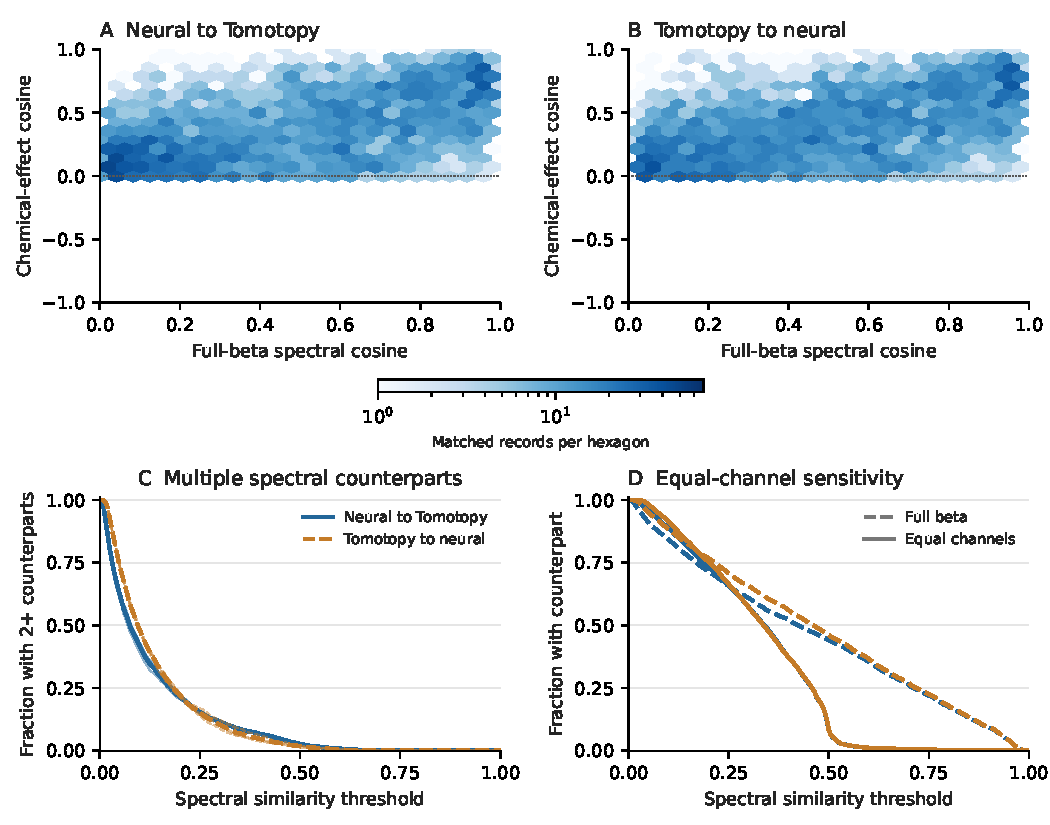
\includegraphics[width=\linewidth]{figures/cross_model_agreement.pdf}
\caption{What cross-model correspondence does and does not establish.
All panels use recurring, evaluable source and target inventories.
(A--B) Full-$\beta$ cosine versus signed MACCS feature-effect cosine for
the closest counterpart; hexagon shading counts fit-pair/topic records on a
shared logarithmic scale. Reused targets and repeated fits make these records
dependent. A includes \OverlapNLChemicalDefined{} records and excludes
\OverlapNLChemicalUndefined{} undefined profile; B includes
\OverlapLNChemicalDefined{} and excludes \OverlapLNChemicalUndefined{}.
These exclusions apply only to chemical agreement, not spectral recovery.
(C) Fraction of source motifs with
at least two counterparts above each threshold; thin lines show source-fit
variation. (D) Mean recovery with full-$\beta$ cosine (dashed) and equal-weight
fragment/loss cosine (solid), with the same directional colors as C.
Spectral multiplicity is not proof of chemical splitting or merging, and
the similarity scales are not probabilities of correct chemistry.}
\label{fig:cross-model-agreement}
\end{figure}
\subsection{Redundancy within each fitted inventory}

Within-fit redundancy also tempers inventory counts. The mean median cosine
to the nearest other topic is \ChemSelectedRedundantMedian{} for the
selected model and \ChemLDARedundantMedian{} for Tomotopy. Exact MAG
consensus profiles recur for \ChemSelectedRepeatedMAG{} and
\ChemLDARepeatedMAG{} topics per fit, respectively
(\ChemSelectedRepeatedMAGPercent{}\% and
\ChemLDARepeatedMAGPercent{}\% of available annotations).
These are repeated coarse fingerprints, not proof that the corresponding
motifs are chemically identical. They nevertheless show why motif count
cannot be read directly as a count of distinct substructures.

\section{Reproducibility and scope of component evidence}
\label{app:repro}

\subsection{Implementation and evidence}
Research code, manuscript sources and versioned evidence are available in the
\href{https://github.com/joewandy/MS2LDA/tree/experiment/minimal-neural-topic-model}{public research branch of the MS2LDA fork}.
The selected implementation is \texttt{reduced\_document\_context} in
\path{benchmarks/neural_ms2lda/contextual_reductions.py}, with shared
mathematical functions in \texttt{contextual\_sparse\_etm.py} and training
through \path{scripts/run_minimal_etm.py}. It remains separate from production
Tomotopy and the archived leave-one-out model.

Historical single-fit reference evidence remains under
\path{research/contextual_sparse_etm_msnlib/evidence/20260901_clean_room/}.
The current three-fit baseline comparison, input identities and source
manifest are under \path{research/baseline_repeats_20260908/evidence/}.

Selected-model evidence consists of nine completed fits, identified by the
selected implementation name in
\path{research/minimal_neural_etm/review_20260907/evidence/within_model/runs.csv}.
Use recorded source snapshots for exact historical replay. A later gradient
correction affects only uniform evidence, a case proved unreachable for the
real and synthetic $K=128$ training inputs but not the $K=36$ trajectories.
Saved results are unchanged; the qualification is documented in
\path{docs/research/equation_code_audit_20260908.md}.

The additional assessment protocol, input seal, full evidence and reproduction
commands are in \path{research/motif_chemical_assessment_20260908/}.
Equations~\ref{eq:sos-excess} and~\ref{eq:feature-enrichment} are implemented
in \path{benchmarks/neural_ms2lda/chemical_nulls.py}, with exhaustive
small-population checks.
Directed recovery (Equation~\ref{eq:directed-recovery}) is implemented in
\path{benchmarks/neural_ms2lda/cross_model_overlap.py}; its sealed evidence,
full replay and denominator audit are in
\path{research/cross_model_overlap_20260908/}. Neither assessment changes
a saved fit or production model.

\subsection{Training settings and random states}
\label{app:recipe}
The canonical environment is \texttt{ms2lda-neural}, specified by the root
\path{environment.yml}; training used PyTorch 2.10.0 with CUDA 12.8.
SGNS uses five epochs, eight count-weighted positive pairs per training
spectrum and five negatives per pair. Negatives follow corpus frequency
raised to $0.75$. SparseAdam uses learning rate $0.01$ and batches of 8,192
pairs. Neural topic-model training uses Adam learning rate $0.005$, moments
$(0.9,0.999)$ and weight decay $1.2\times10^{-6}$, with 120 epochs and batch
size 200. The plain-ETM reference uses batch size 256.

The real-data partition uses random state 42. Selected real training seeds
are 7012, 7024 and 7043, corresponding to run labels 11, 23 and 42.
Plain ETM uses the same training seeds; only its last fit is historical.
Tomotopy uses seeds 11, 23 and 42. Synthetic realization seeds are 11, 23
and 37, with training seeds 7012, 7024 and 7038 at both fitted topic counts.
Within each real-data model, data partitions, vocabulary, embeddings and fitting
settings are fixed across repetitions. No selected-model fit was rerun.
The original plain-ETM fit ran under WSL2, whereas its two new repetitions
ran on native Linux. Both use an RTX 5070 and matching recorded versions of
the scientific packages, including PyTorch 2.10.0 with CUDA 12.8; the Python
build and operating environment differ. The baseline bundle preserves both
environment records. Its SD is therefore across fitted runs, not an isolated
estimate of seed-only variation.

Generate the audited result fragments and run the scientific checks from
the repository root:
\begin{quote}\small\ttfamily
python -S -m scripts.generate\_contextual\_reduction\_review\\
python -m scripts.generate\_motif\_chemical\_assessment\_report\\
python -m scripts.generate\_cross\_model\_overlap\_report\\
pytest -q benchmarks/neural\_ms2lda/tests
\end{quote}
Compile both the main paper and this supplement from \path{docs/research/},
making their auxiliary files available through \texttt{TEXINPUTS}. Alternate
\texttt{pdflatex} passes until cross-document references stabilize, then render
and inspect every PDF page. The repository report README gives the full recipe. Probability,
gradient and checkpoint-reload tests check that the reported equations match
the chosen implementation. Per-run records remain in the research archive.

\subsection{Scope of the existing component evidence}
\label{app:ablations}
In one paired real-data comparison of the closely related leave-one-out
predecessor, removing channel balancing reduced useful motifs from 394 to 322.
Restoring softmax
in the within-model screen retained useful-motif breadth but produced much
more diffuse mixtures, supporting entmax's compactness role. Comparisons with
context-free variants support the context pathway under the tested training
settings, but do not establish that
all spectra or all neural topic models require that pathway. Removing an
entire evidence branch and removing only contextual mixing are different
interventions and must not be conflated.

These are development comparisons, not factorial ablations of the final model.
Whole-spectrum context preserved the discovery/compactness trade-off in three
paired predecessor comparisons. The complete records are linked from the
source inventory; they do not establish global model minimality.
\clearpage
% Shared bibliography for the main paper and supplementary information.
\begin{thebibliography}{99}
\bibitem{vanderhooft2016}
J. J. J. van der Hooft, J. Wandy, M. P. Barrett, K. E. V. Burgess, and
S. Rogers. \emph{Topic modeling for untargeted substructure exploration in
metabolomics}. PNAS 113, 13738--13743 (2016).
\url{https://doi.org/10.1073/pnas.1608041113}

\bibitem{torresortega2026}
L. R. Torres Ortega et al. \emph{Large-scale discovery and annotation of
substructure patterns in mass spectrometry profiles}.
Nature Communications 17, 8350 (2026).
\url{https://doi.org/10.1038/s41467-026-75038-0}

\bibitem{blei2003}
D. M. Blei, A. Y. Ng, and M. I. Jordan. \emph{Latent Dirichlet Allocation}.
JMLR 3, 993--1022 (2003).
\url{https://jmlr.org/papers/v3/blei03a.html}

\bibitem{dieng2020}
A. B. Dieng, F. J. R. Ruiz, and D. M. Blei. \emph{Topic Modeling in Embedding
Spaces}. TACL 8, 439--453 (2020).
\url{https://doi.org/10.1162/tacl_a_00325}

\bibitem{srivastava2017}
A. Srivastava and C. Sutton. \emph{Autoencoding Variational Inference for
Topic Models}. ICLR (2017).
\url{https://openreview.net/forum?id=BybtVK9lg}

\bibitem{mikolov2013}
T. Mikolov et al. \emph{Distributed Representations of Words and Phrases
and their Compositionality}. NeurIPS (2013).
\href{https://proceedings.neurips.cc/paper/2013/hash/9aa42b31882ec039965f3c4923ce901b-Abstract.html}{NeurIPS proceedings entry.}

\bibitem{huber2021}
F. Huber et al. \emph{Spec2Vec: Improved mass spectral similarity scoring
through learning of structural relationships}. PLOS Computational Biology 17,
e1008724 (2021).
\url{https://doi.org/10.1371/journal.pcbi.1008724}

\bibitem{peters2019}
B. Peters, V. Niculae, and A. F. T. Martins. \emph{Sparse Sequence-to-Sequence
Models}. ACL, 1504--1519 (2019).
\url{https://doi.org/10.18653/v1/P19-1146}

\bibitem{brungs2025}
C. Brungs et al. \emph{MS$^{n}$Lib: efficient generation of open multi-stage
fragmentation mass spectral libraries}. Nature Methods 22, 2028--2031 (2025).
\url{https://doi.org/10.1038/s41592-025-02813-0}

\bibitem{msnlibdata}
J. Dietrich, J. Wandy, L. R. Torres Ortega, and J. J. J. van der Hooft.
\emph{vdhooftcompmet/MS2LDA: Paper---Data and Models}. Zenodo (2026).
\url{https://doi.org/10.5281/zenodo.20179680}

\bibitem{bemismurcko1996}
G. W. Bemis and M. A. Murcko. \emph{The Properties of Known Drugs. 1.
Molecular Frameworks}. Journal of Medicinal Chemistry 39, 2887--2893 (1996).
\url{https://doi.org/10.1021/jm9602928}

\bibitem{durant2002}
J. L. Durant, B. A. Leland, D. R. Henry, and J. G. Nourse.
\emph{Reoptimization of MDL Keys for Use in Drug Discovery}.
Journal of Chemical Information and Computer Sciences 42, 1273--1280 (2002).
\url{https://doi.org/10.1021/ci010132r}

\bibitem{tomotopy}
M. Lee. \emph{Tomotopy}, release 0.13.0 (2024).
\href{https://github.com/bab2min/tomotopy/releases/tag/v0.13.0}{Official release v0.13.0.}

\bibitem{rogers2019}
S. Rogers, C. W. Ong, J. Wandy, M. Ernst, L. Ridder, and J. J. J. van der Hooft.
\emph{Deciphering complex metabolite mixtures by unsupervised and supervised
substructure discovery and semi-automated annotation from MS/MS spectra}.
Faraday Discussions 218, 284--302 (2019).
\url{https://doi.org/10.1039/C8FD00235E}

\bibitem{panwar2021}
M. Panwar, S. Shailabh, M. Aggarwal, and B. Krishnamurthy.
\emph{TAN-NTM: Topic Attention Networks for Neural Topic Modeling}.
ACL-IJCNLP, 3865--3880 (2021).
\url{https://doi.org/10.18653/v1/2021.acl-long.299}

\bibitem{bushuiev2026}
R. Bushuiev et al. \emph{Self-supervised learning of molecular representations
from millions of tandem mass spectra using DreaMS}.
Nature Biotechnology 44, 630--640 (2026; published online 2025).
\url{https://doi.org/10.1038/s41587-025-02663-3}

\bibitem{pyroprodlda}
Pyro contributors. \emph{Probabilistic Topic Modeling: ProdLDA}.
Official Pyro tutorial, accessed 8 September 2026.
\url{https://pyro.ai/examples/prodlda.html}
\bibitem{phipson2010}
B. Phipson and G. K. Smyth. \emph{Permutation P-values should never be zero:
calculating exact P-values when permutations are randomly drawn}.
Statistical Applications in Genetics and Molecular Biology 9, Article 39 (2010).
\url{https://doi.org/10.2202/1544-6115.1585}

\bibitem{benjamini2001}
Y. Benjamini and D. Yekutieli. \emph{The control of the false discovery rate
in multiple testing under dependency}. Annals of Statistics 29,
1165--1188 (2001).
\url{https://doi.org/10.1214/aos/1013699998}
\end{thebibliography}

\end{document}
